\documentclass[12pt]{article}
\usepackage{amsmath, amssymb, amsthm}
\usepackage{mathtools}
\usepackage{graphicx}
\usepackage{float}
\usepackage{hyperref}
\usepackage{xcolor}
\usepackage{listings}
\usepackage{geometry}
\usepackage{algorithm}
\usepackage{algpseudocode}
\usepackage{tikz}
\usepackage{longtable}

% Page Setup
\geometry{a4paper, margin=1in}

\newcommand{\vecb}[1]{\mathbf{#1}}
\newcommand{\brak}[1]{\ensuremath{\left(#1\right)}}
\newcommand{\cbrak}[1]{\ensuremath{\left\{#1\right\}}}
\newcommand{\abs}[1]{\left\vert#1\right\vert}
\newcommand{\norm}[1]{\left\lVert#1\right\rVert}

\begin{document}

\bibliographystyle{IEEEtran}
\vspace{3cm}

\title{Lissajous Figures and One-Time events on Oscilloscopes\\\brak{\text{EE1200 - Lab 1 Report}}}
\author{Abhimanyu Koushik \brak{\text{EE24BTECH11024}},\\Agamjot Singh \brak{\text{EE24BTECH11002}}\\IIT Hyderabad}
{\let\newpage\relax\maketitle}

\renewcommand{\thefigure}{\theenumi}
\renewcommand{\thetable}{\theenumi}
\setlength{\intextsep}{10pt} % Space between text and floats

\numberwithin{equation}{enumi}
\numberwithin{figure}{enumi}
\renewcommand{\thetable}{\theenumi}

\section{Introduction}
Lissajous figures are used for periodic signals where the relationship between two waveforms (e.g., their phase, amplitude, and frequency ratio) is to be visualized in the $X$-$Y$ mode of an oscilloscope. In simple terms, these figures are curves obtained when two periodic signals are applied to the horizontal and vertical inputs of an oscilloscope. These figures depend on the frequency ratio, amplitude ratio, and phase difference of the two signals.

\subsection{Objective}
The purpose of this experiment is to:
\begin{itemize}
    \item Generate Lissajous figures using a function generator.
    \item Analyze the effect of frequency ratio and phase difference on the shapes of the figures.
\end{itemize}

\section{Materials and Methods}
\subsection{Equipment Used}
\begin{itemize}
    \item Function generator
    \item Oscilloscope
    \item BNC cables
    \item Probes
\end{itemize}

\subsection{Procedure (Lissajous Figures)}
\begin{enumerate}
    \item Connect the function generator to the oscilloscope using BNC cables to the probes of the oscilloscope's probes.
    The ground (black) wire of the BNC cable is the ground which is to be connected to the ground of the probe (which is sticking out). The live (red) wire of the BNC cable is to be connected to the probe.
    \item Set the function generator to produce two periodic signals $x\brak{t}$ and $y\brak{t}$ of certain frequency and phase difference.
    \item Connect both the BNC cables \brak{x \text{ and } y \text{ representing } x\brak{t} \text{ and } y\brak{t} \text{ respectively}} to channel $1$ and $2$ of the oscilloscope respectively.
    \item Set the display mode to $X - Y$ and align the phase after each change in the \textbf{Inter CH} dropdown.
    \item Vary the frequency ratio and phase difference between the two signals to observe changes in the Lissajous figures.
    \item Record the observations and capture the figures displayed on the oscilloscope.
\end{enumerate}

\section{Theory}

Let the general parametric equations for Lissajous figures be given by,
\begin{align}
    x &= x\brak{t}\\
    y &= y\brak{t}\\
\end{align}
For a given parameter $t_0$, $x\brak{t_0}$ and $y\brak{t_0}$ are plotted on the $x$-axis and $y$-axis respectively.
\newline
\newline
The shape of the Lissajous figure is determined by the type of waveforms $x\brak{t}$, $y\brak{t}$, frequency ratio $\brak{\dfrac{\omega_x}{\omega_y}}$, the amplitude ratio $\brak{\dfrac{A}{B}}$ and the phase difference $\Delta \phi = \phi_x - \phi_y$, where
\begin{itemize}
    \item $A$ and $B$ are the amplitudes of the signals.
    \item $\omega_x$ and $\omega_y$ are the angular frequencies.
    \item $\phi_x$ and $\phi_y$ are the initial phases.
\end{itemize}

\section{Capturing One-Time Events}
\begin{enumerate}
    \item Connection of the BNC cables with the probes is same as before. Except for this time only one channel (channel 1) is connected between the function generator and the oscilloscope.
    \item The mode of the function generator is to be shifted to the \textbf{Burst Mode} and the trigger is to be set the \textbf{Manual Trigger}.
    \item Number of cycles of the waveform are to be appropriately selected.
    \item The oscilloscope's coupling should be set DC, and the sweep should be set to \textbf{Normal}. The trigger mode should be set as \textbf{Edge} with the channel as channel $1$.
    \item First we switch the mode of the oscilloscope to \textbf{Single} and set the trigger level to an appropriate level.
    \item We then push the knob on the function generator to manually trigger the one-time event which is captured on the oscilloscope.
\end{enumerate}

\section{Results}
\begin{figure*}[ht!]
    {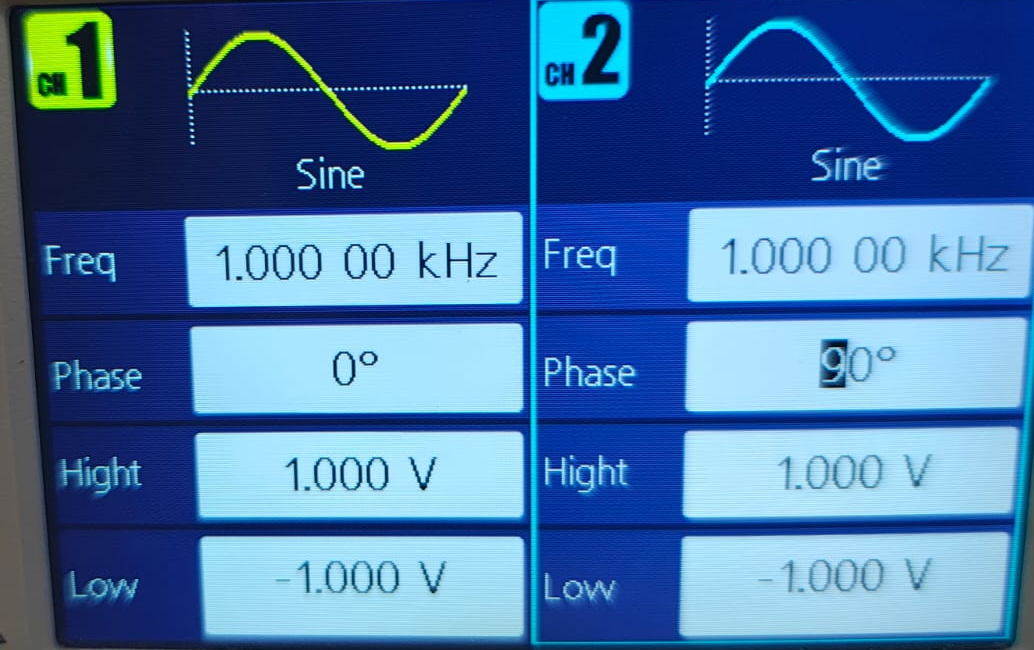
\includegraphics[ width=0.31\textwidth]{./figs/data1_crop.png}}
    \hspace{\fill}
    {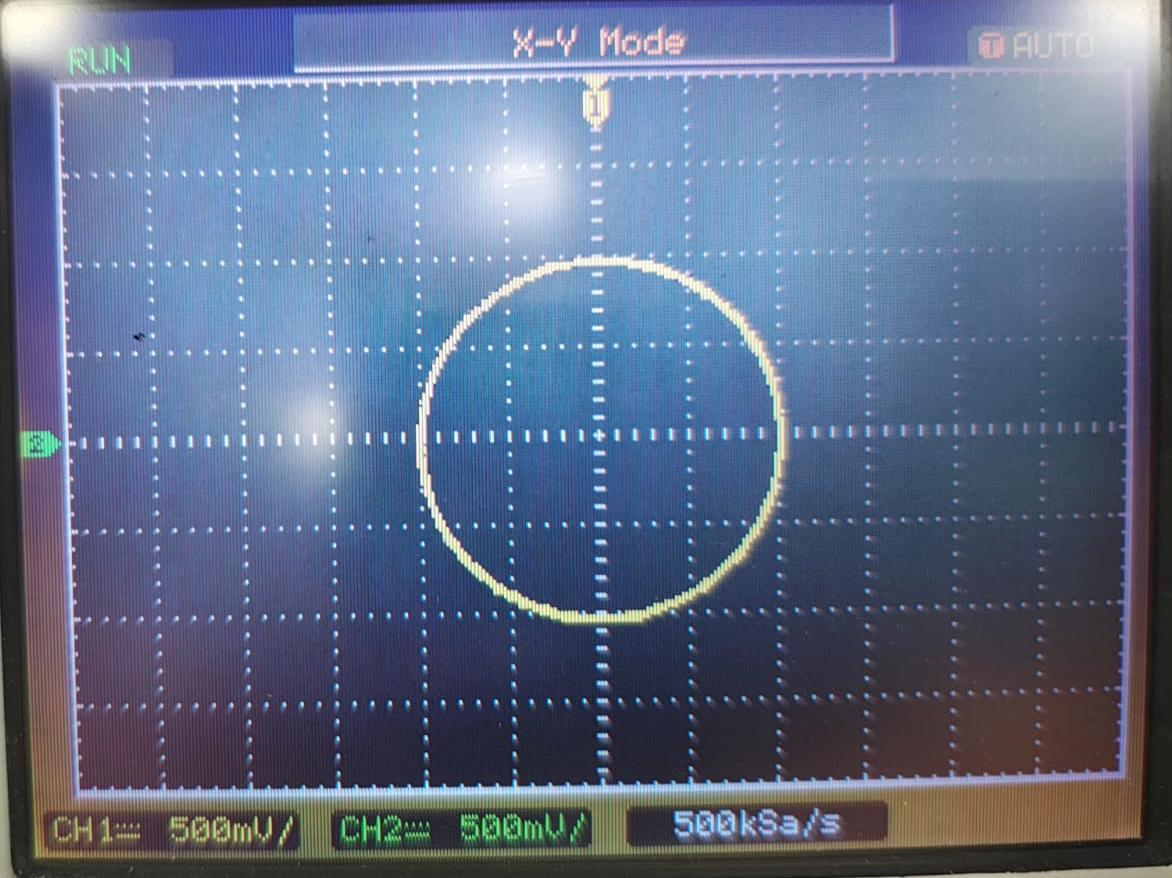
\includegraphics[ width=0.31\textwidth]{./figs/fig1_crop.png}}
    \hspace{\fill}
    {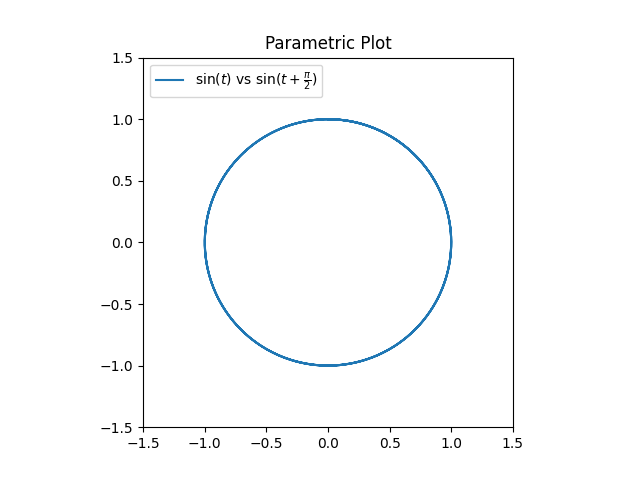
\includegraphics[ width=0.31\textwidth]{./figs/fig1_verify.png}}\\
    \caption{Lissajous Plot 1}
\end{figure*}
\begin{figure*}[ht!]
    {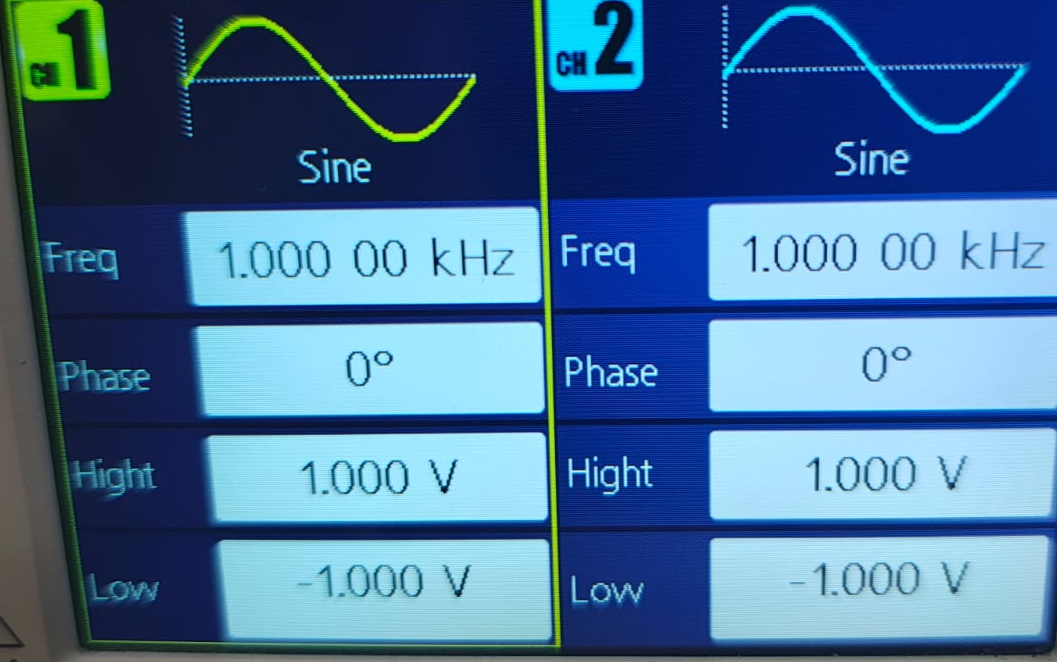
\includegraphics[ width=0.31\textwidth]{./figs/data2_crop.png}}
    \hspace{\fill}
    {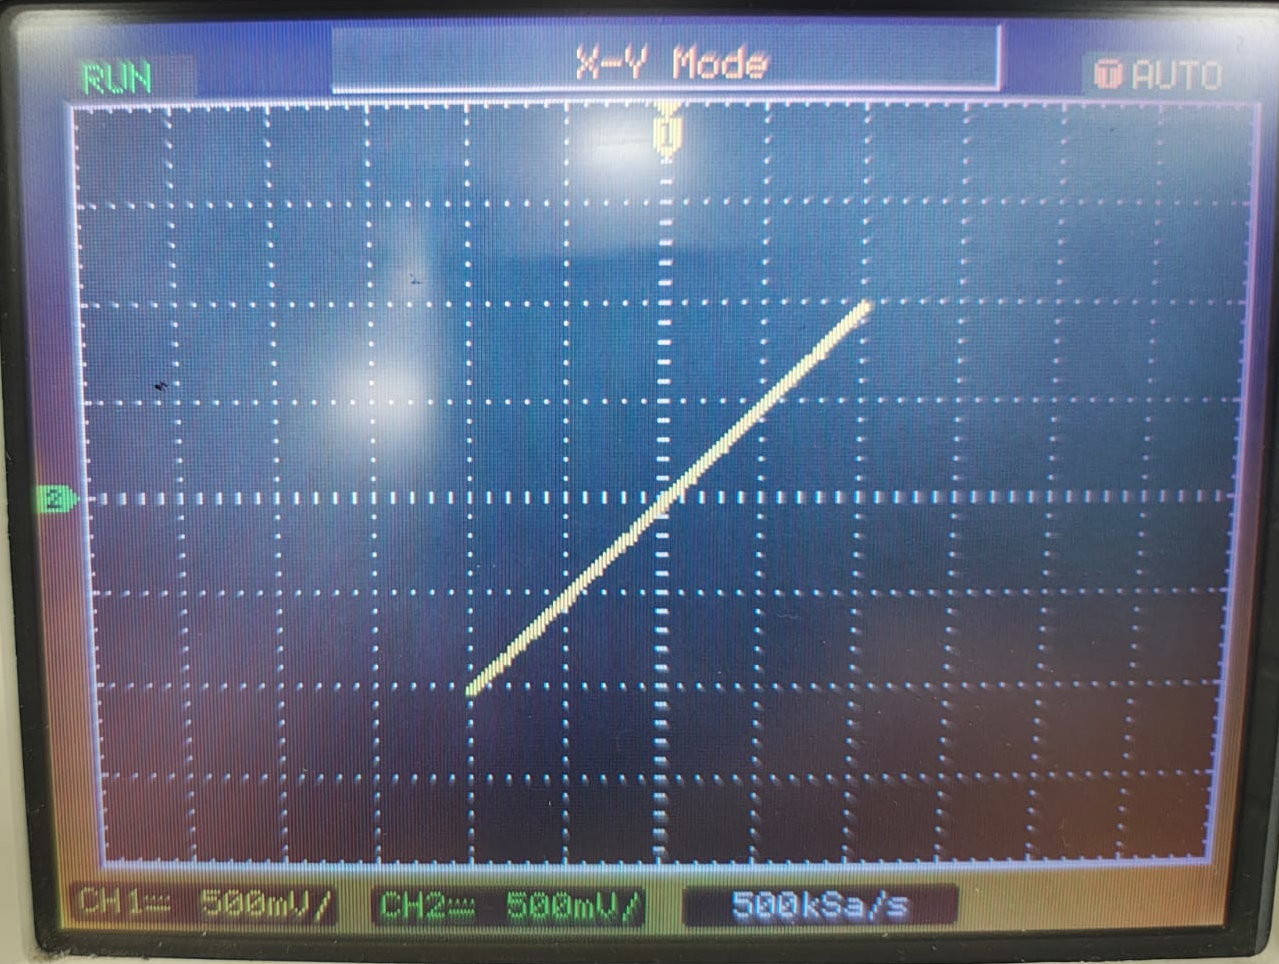
\includegraphics[ width=0.31\textwidth]{./figs/fig2_crop.png}}
    \hspace{\fill}
    {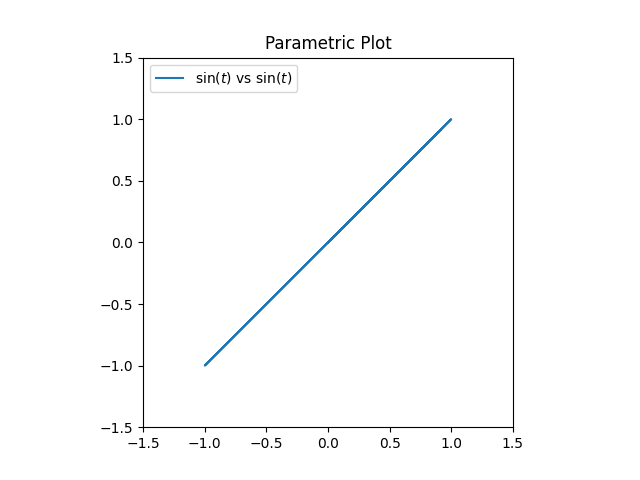
\includegraphics[ width=0.31\textwidth]{./figs/fig2_verify.png}}\\
    \caption{Lissajous Plot 2}
\end{figure*}
\begin{figure*}[ht!]
    {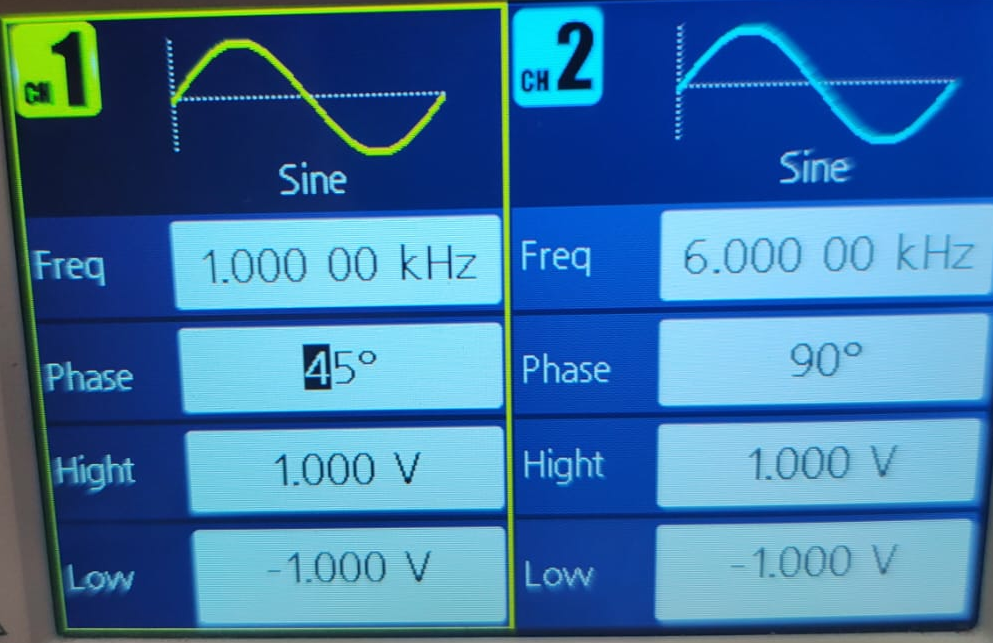
\includegraphics[ width=0.31\textwidth]{./figs/data3_crop.png}}
    \hspace{\fill}
    {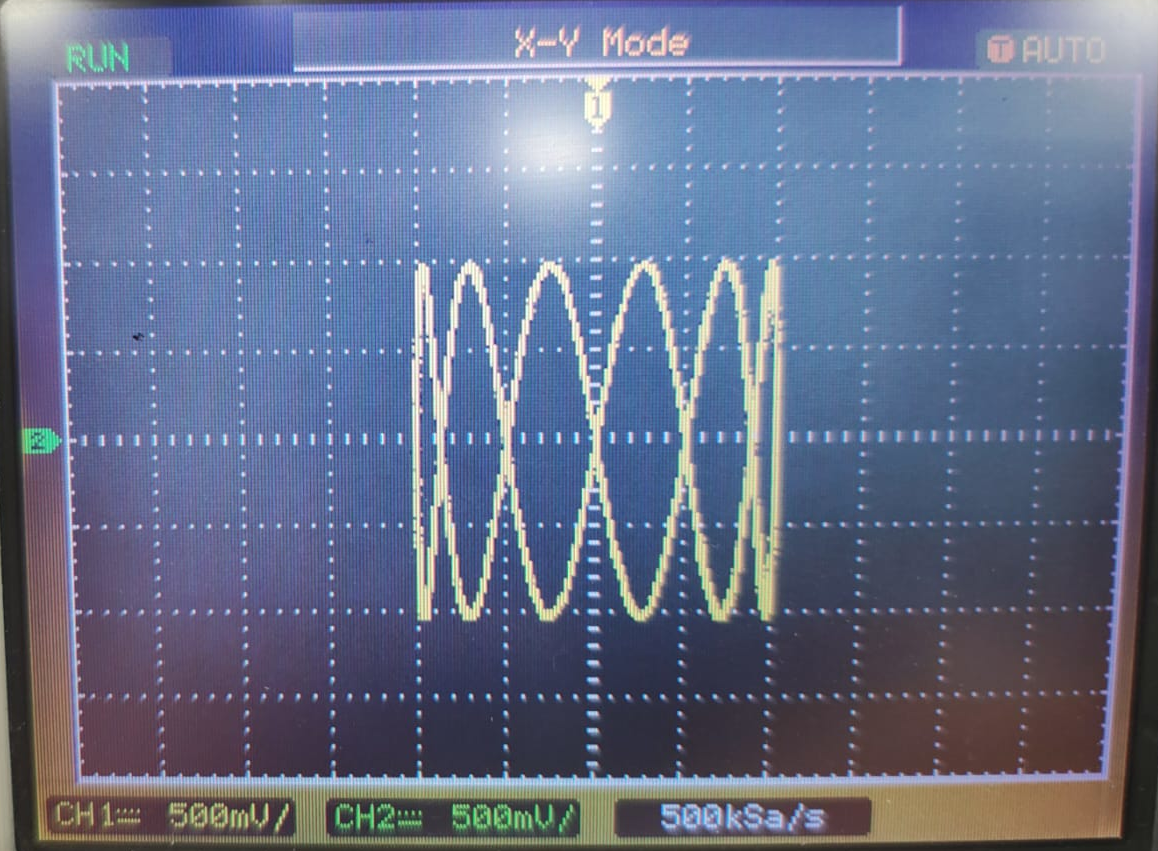
\includegraphics[ width=0.31\textwidth]{./figs/fig3_crop.png}}
    \hspace{\fill}
    {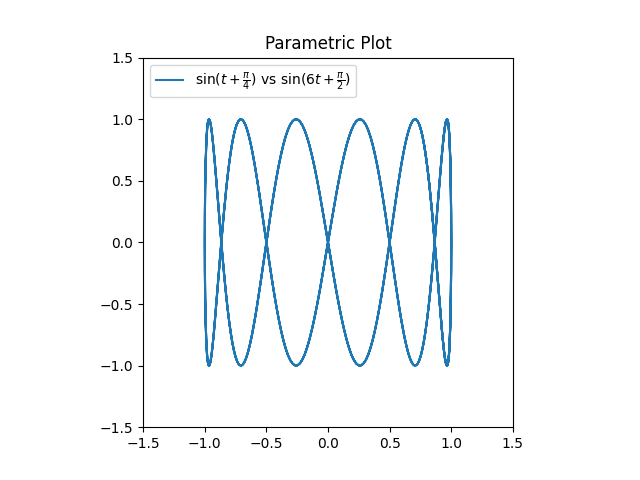
\includegraphics[ width=0.31\textwidth]{./figs/fig3_verify.png}}\\
    \caption{Lissajous Plot 3}
\end{figure*}
\begin{figure*}[ht!]
    {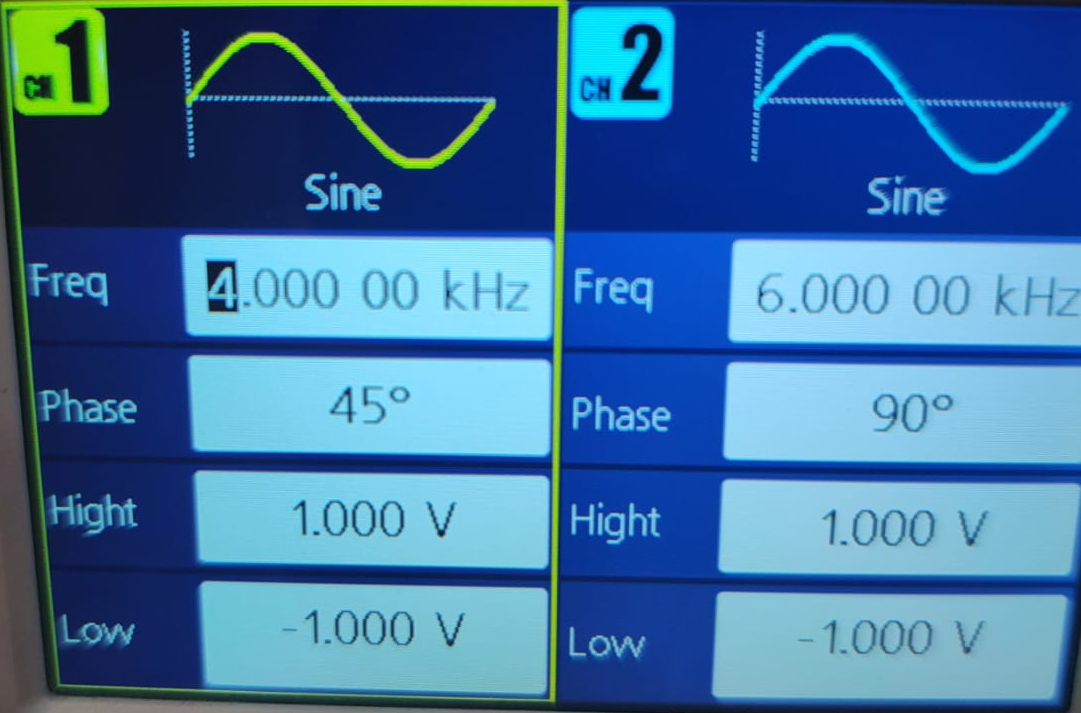
\includegraphics[ width=0.31\textwidth]{./figs/data4_crop.png}}
    \hspace{\fill}
    {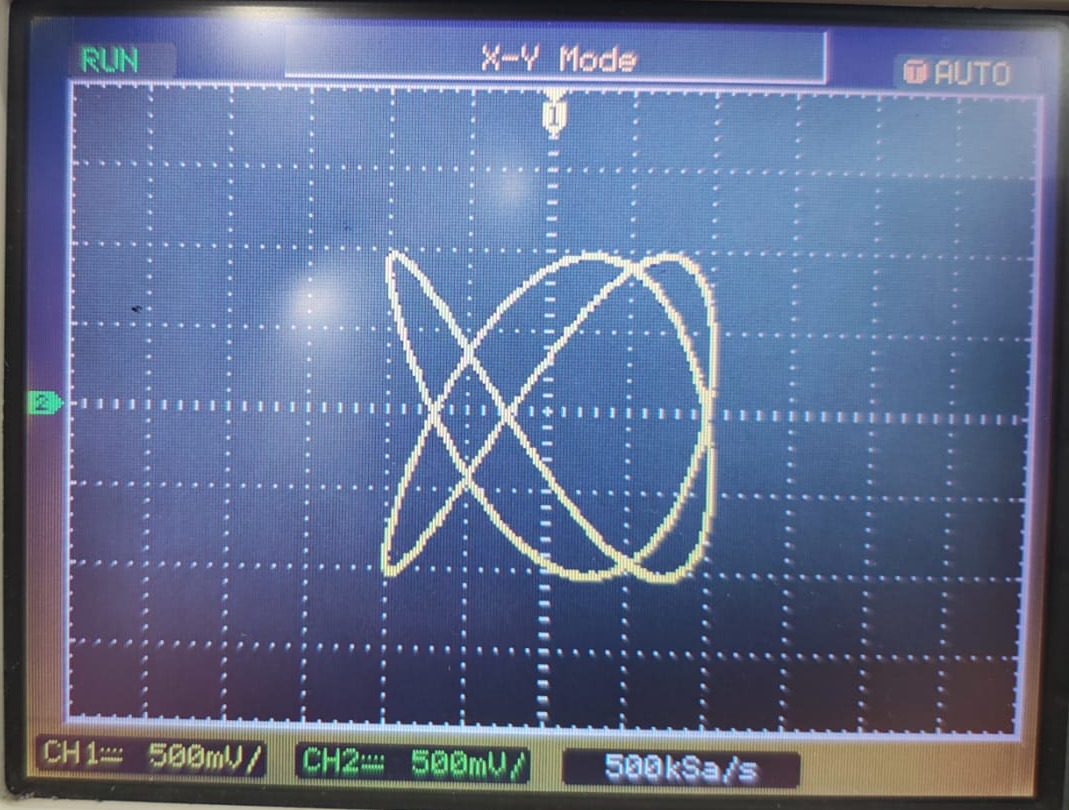
\includegraphics[ width=0.31\textwidth]{./figs/fig4_crop.png}}
    \hspace{\fill}
    {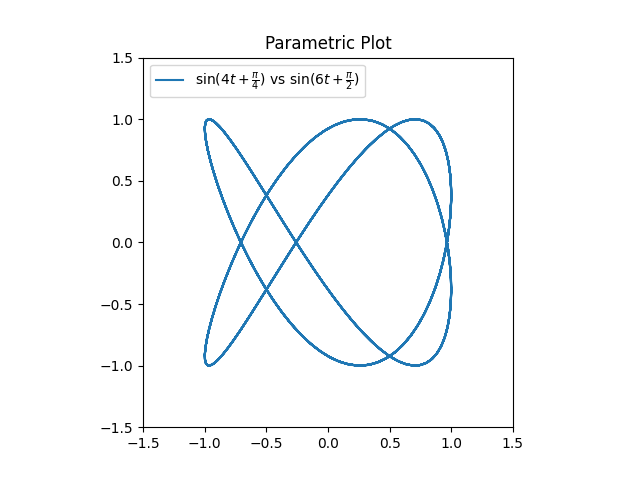
\includegraphics[ width=0.31\textwidth]{./figs/fig4_verify.png}}\\
    \caption{Lissajous Plot 4}
\end{figure*}
\begin{figure*}[ht!]
    {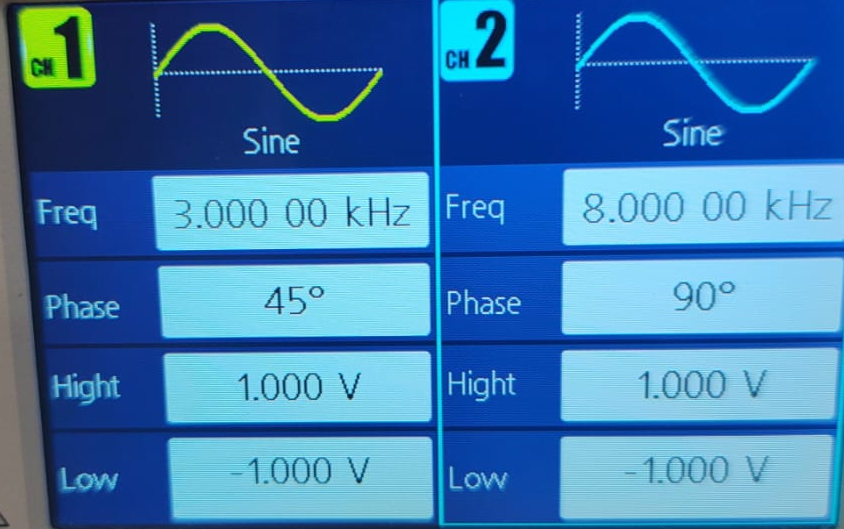
\includegraphics[ width=0.31\textwidth]{./figs/data5_crop.png}}
    \hspace{\fill}
    {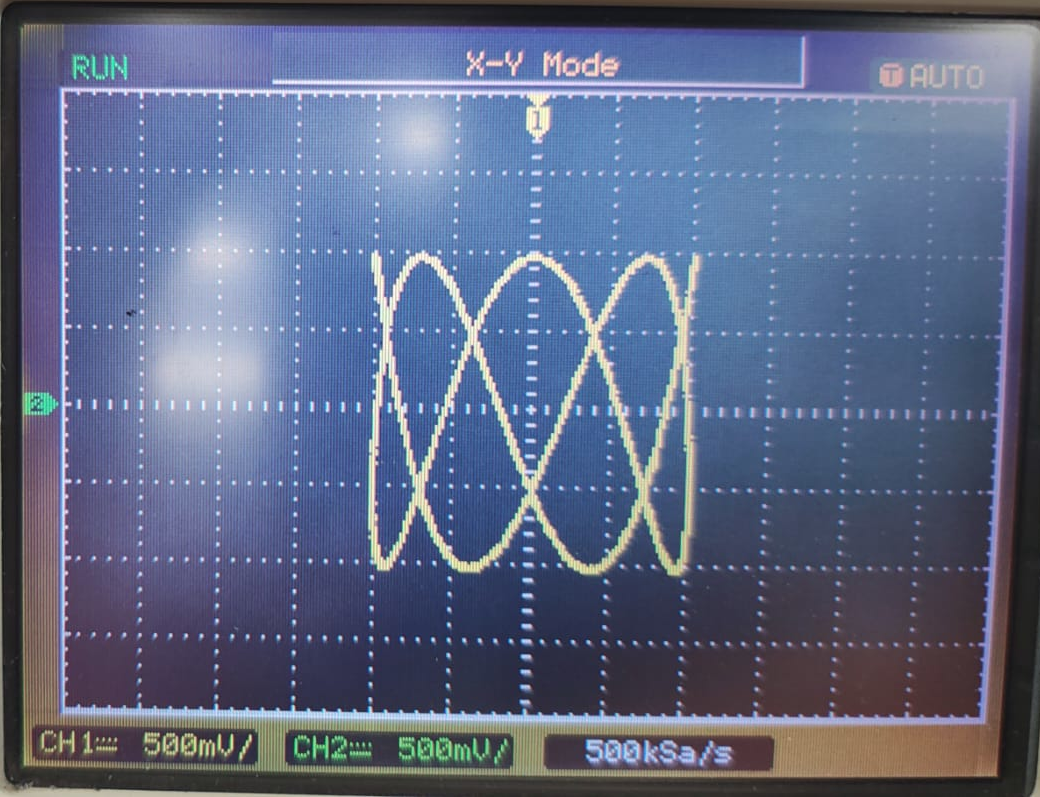
\includegraphics[ width=0.31\textwidth]{./figs/fig5_crop.png}}
    \hspace{\fill}
    {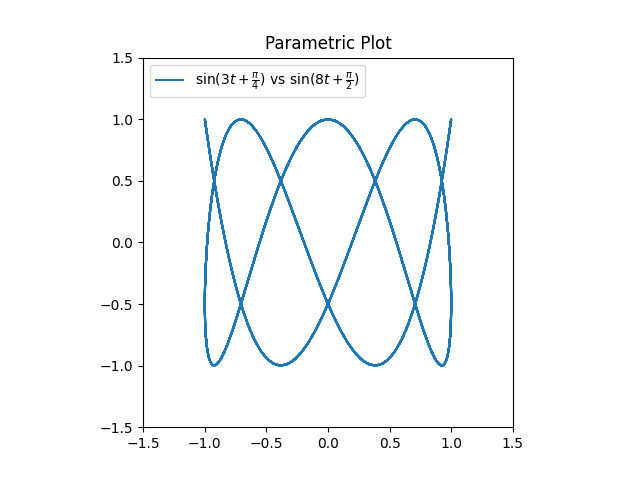
\includegraphics[ width=0.31\textwidth]{./figs/fig5_verify.png}}\\
    \caption{Lissajous Plot 5}
\end{figure*}
\begin{figure*}[ht!]
    {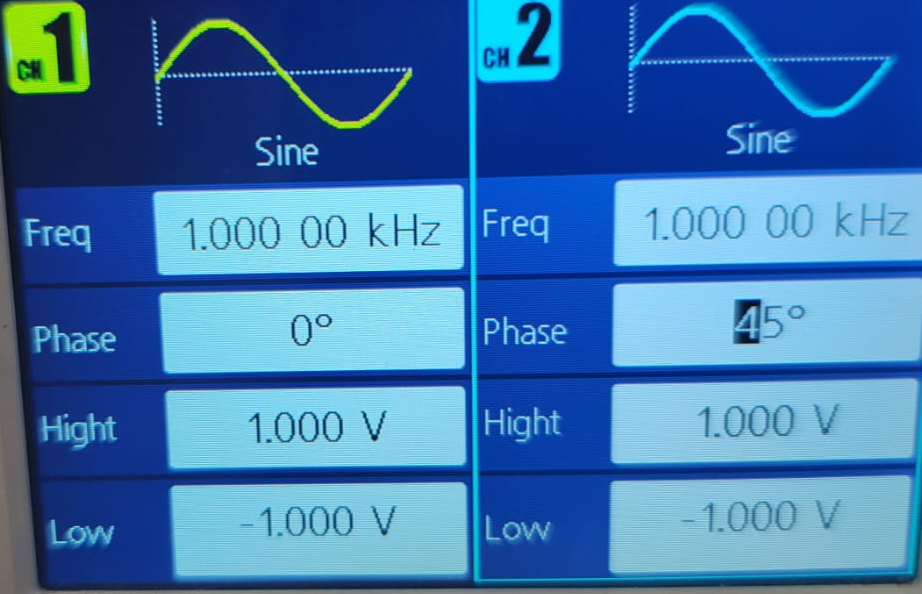
\includegraphics[ width=0.31\textwidth]{./figs/data6_crop.png}}
    \hspace{\fill}
    {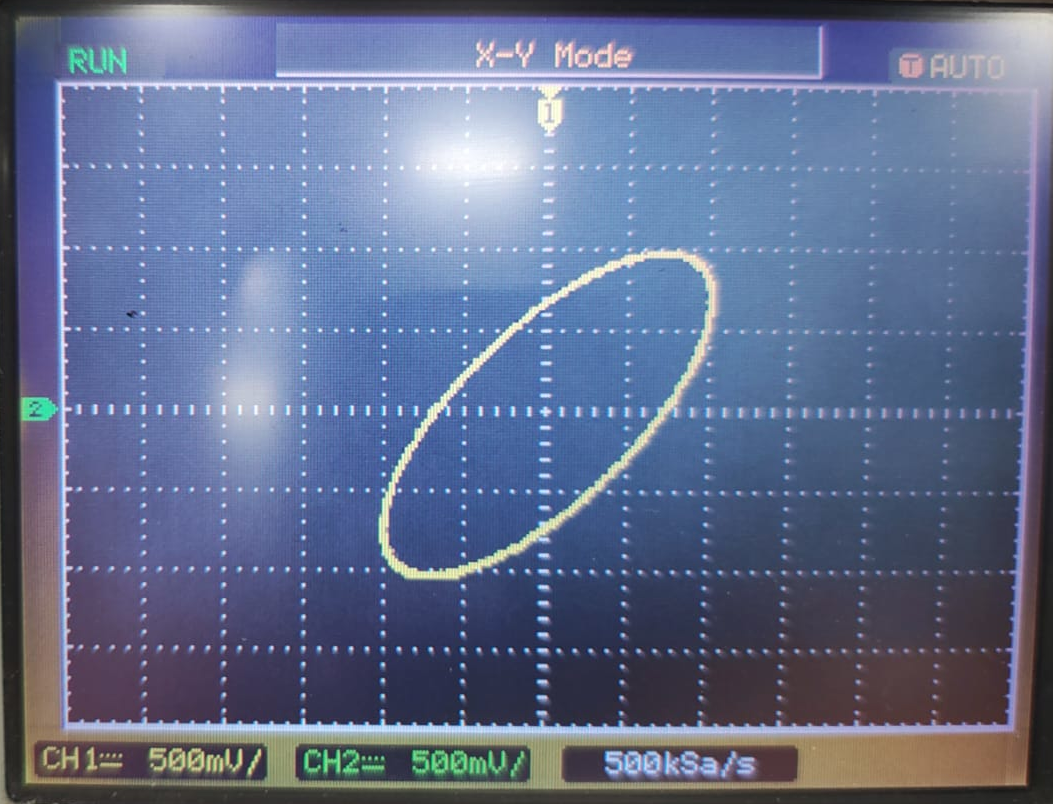
\includegraphics[ width=0.31\textwidth]{./figs/fig6_crop.png}}
    \hspace{\fill}
    {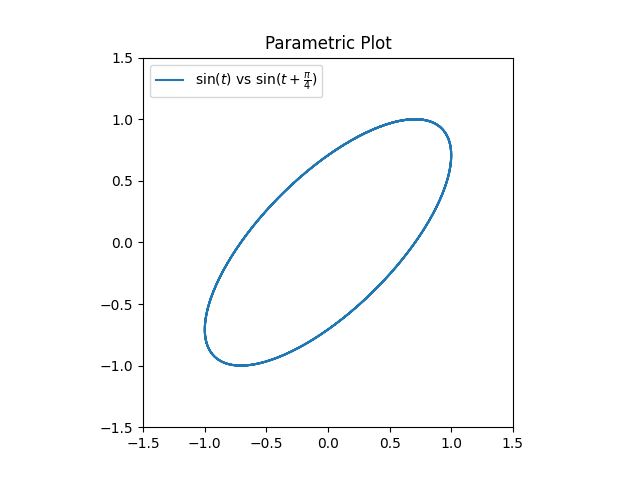
\includegraphics[ width=0.31\textwidth]{./figs/fig6_verify.png}}\\
    \caption{Lissajous Plot 6}
\end{figure*}
\begin{figure*}[ht!]
    {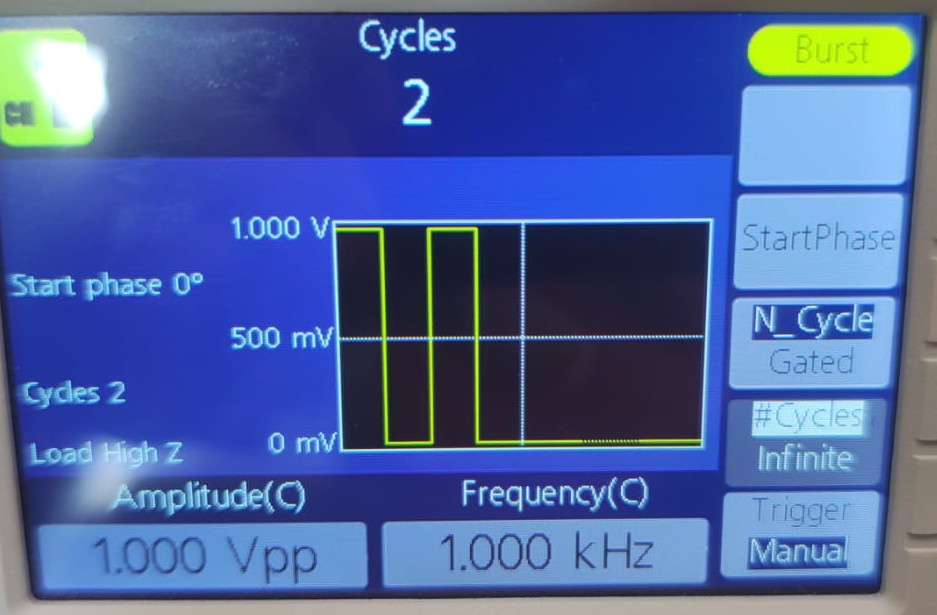
\includegraphics[ width=0.5\textwidth]{./figs/one_time_data_crop.jpeg}}
    \hspace{\fill}
    {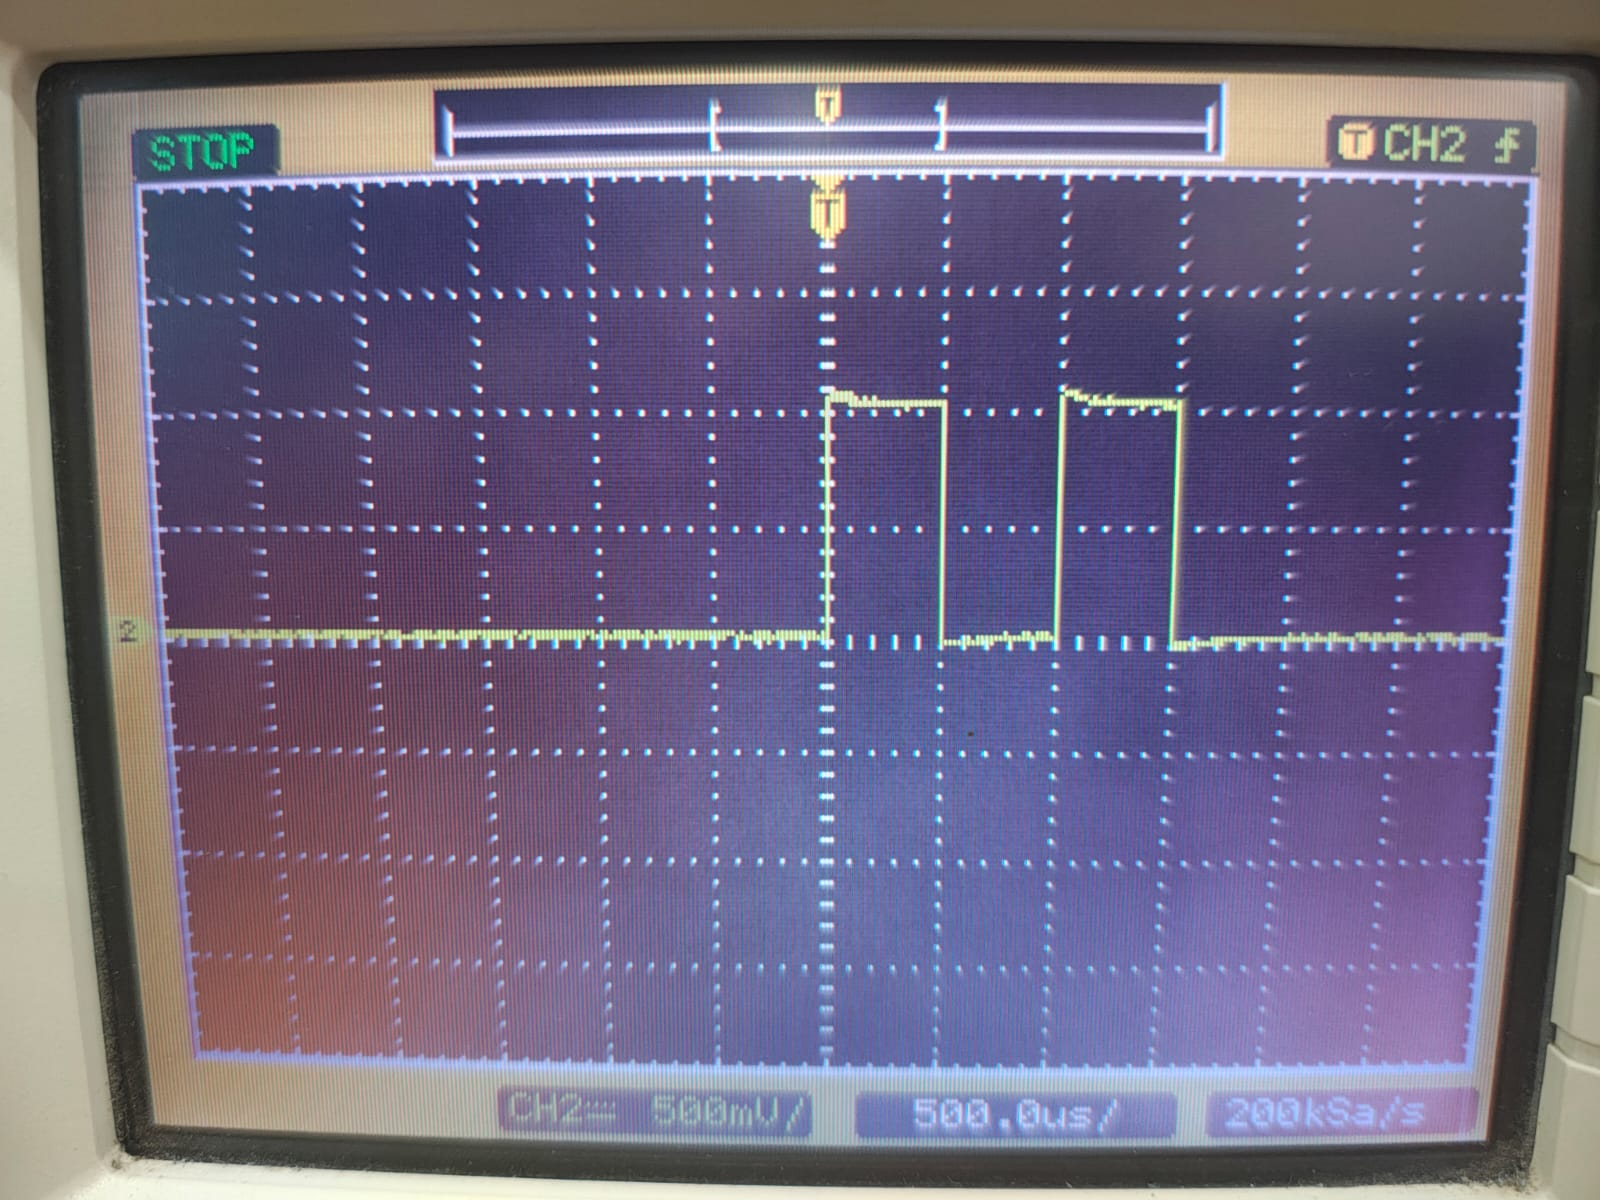
\includegraphics[ width=0.5\textwidth]{./figs/one_time_fig.jpeg}}
    \caption{One-Time Event Plot}
\end{figure*}

\section{Discussion}
The results demonstrate that:
\begin{itemize}
    \item A frequency ratio of $1$ produces simple figures like straight lines, circles or ellipses, depending on the phase difference.
    \item Non-integer frequency ratios produce more complex and interesting figures.
    \item Phase differences shift the orientation and symmetry of the patterns.
\end{itemize}

\section{Conclusion}
Lissajous figures are a powerful tool for visualizing and analyzing the relationship between two periodic signals. The experiment tries to analyze the dependence of these figures on frequency and amplitude ratios and phase differences.

\end{document}
